\section{Data collection}
As our activity deals with thermal images of different bandwidths, there were no off-the-shelf datasets available for training and testing our proposed method.
The only remotely related available datasets were of satellite missions, but those are not open-sourced and only provide post-processed data (\eg, estimated humidity) maps rather than raw thermal images.
Therefore, we decided to assemble a dedicated dataset in-house.

Since most thermal imaging for agricultural purposes is performed by satellites, our goal was to mimic the interstellar acquisition setup to the best of our ability.
To that end, a light airplane (appears in figure \ref{fig:light_airplane}) was used to perform flights at a height of approximately two kilometers above ground.
\begin{figure}[H]
    \centering
    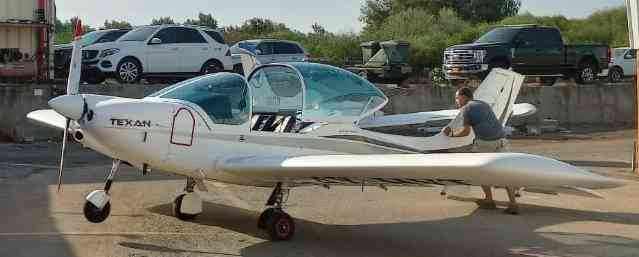
\includegraphics[width=0.8\linewidth]{../figs/data/light_airplane.jpeg}
    \caption{The light airplane used for acquiring the thermal images.}
    \label{fig:light_airplane}
\end{figure}
Images acquired in such a setup could be later reasonably extrapolated, \eg, by a proper downsampling, to mimic the scene as if it was captured by an actual satellite.
A dedicated jig was designed and manufactured to mount the camera on the airplane's underbelly, as visualized in figure \ref{fig:camera_jig}.
\begin{figure}[H]
    \begin{subfigure}[b]{0.49\textwidth}
        \centering
        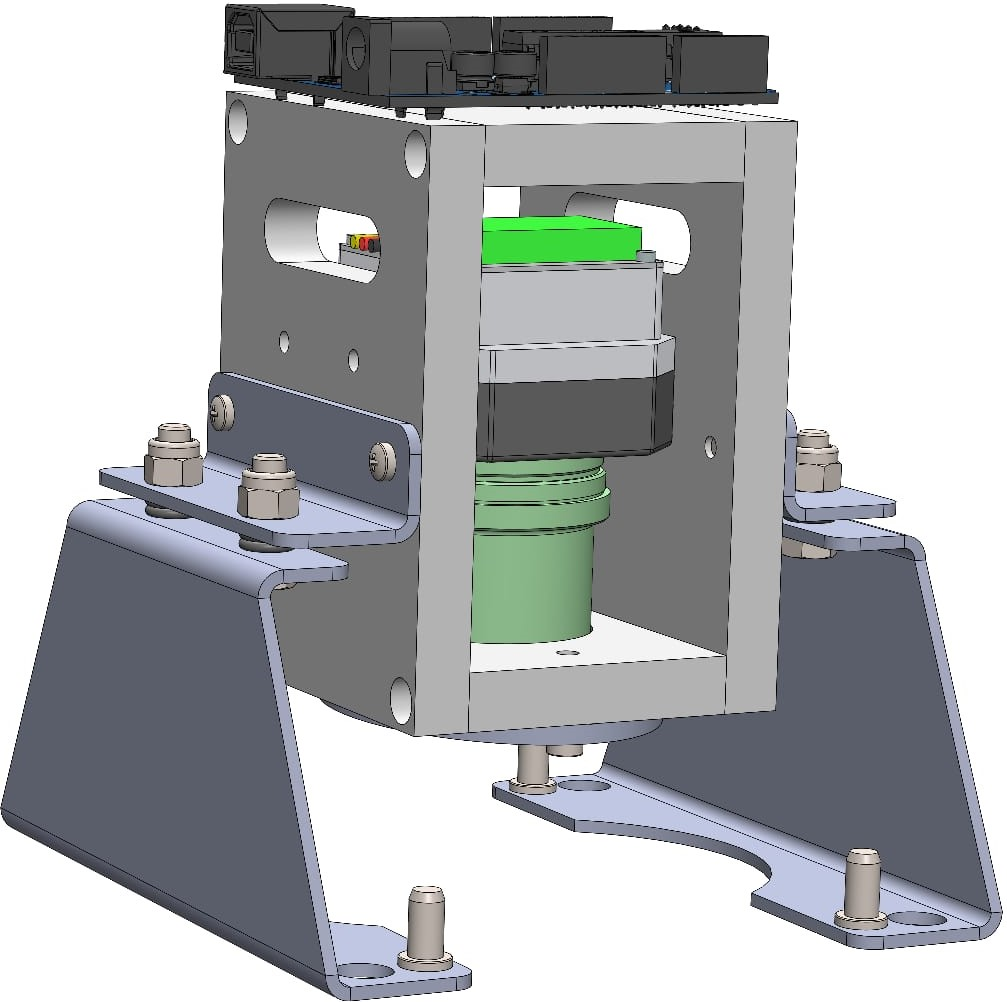
\includegraphics[width=\textwidth]{../figs/data/camera_jig_design.jpeg}
        \subcaption{Design}
        \label{fig:design}
    \end{subfigure}
    \hfill
    \begin{subfigure}[b]{0.49\textwidth}
        \centering
        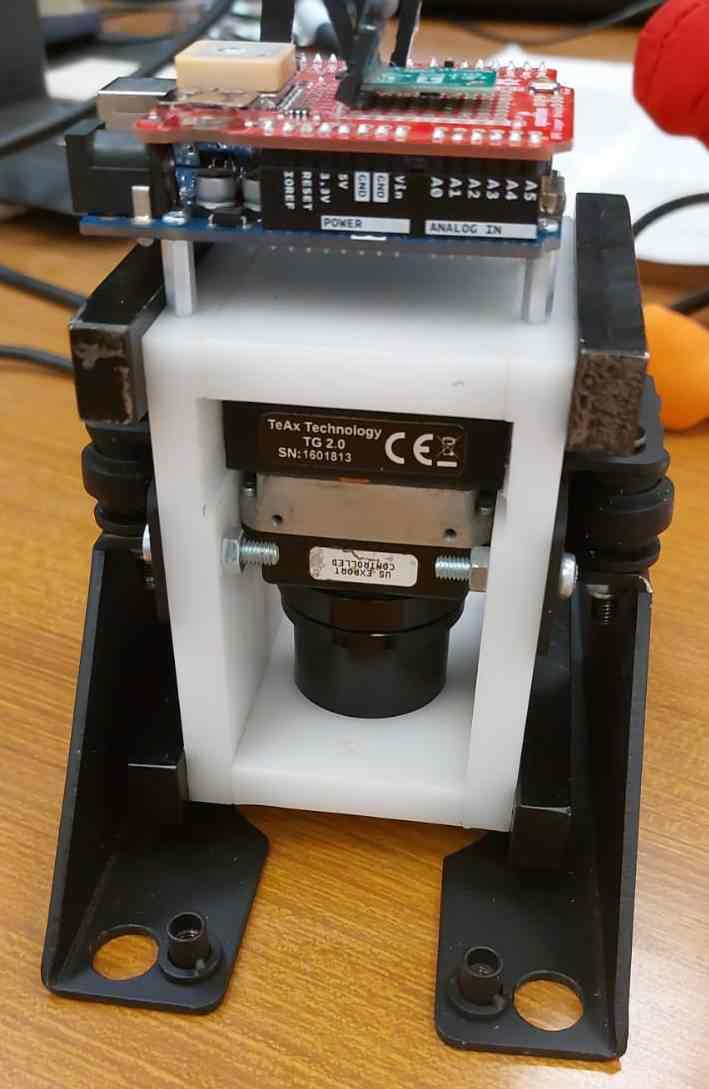
\includegraphics[width=\textwidth]{../figs/data/camera_jig_actual.jpeg}
        \subcaption{Manufactured}
        \label{fig:manufactured}
    \end{subfigure}

    \caption{The design and the eventually manufactured jig for mounting the thermal camera on the light airplane's underbelly.}
    \label{fig:camera_jig}
\end{figure}

Since our research requires both monochromatic and panchromatic images, the pilot performed several flights, with a $9 \mu m$ IR bandpass filter applied to the camera lens, or without this filter.
Each flight attempted to cover the same rectangular ground patch by following a raster trajectory, as demonstrated in figure \ref{fig:aerial_strip}.
\begin{figure}[H]
    \centering
    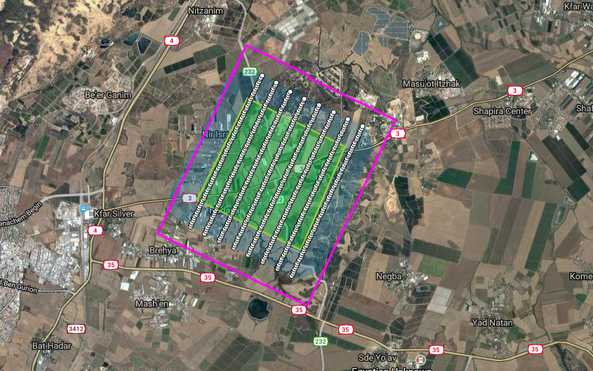
\includegraphics[width=\linewidth]{../figs/data/aerial_strip.jpeg}
    \caption{An illustration of a rectangular ground patch coverage by a raster trajectory}
    \label{fig:aerial_strip}
\end{figure}
Even when attempting to follow the predefined trajectory, ensuring that the actual airplane's positional and angular states are the same for two different flights is physically infeasible.
In addition, jittering and air bumps provide additional randomness to the system's state, resulting in unpredictable and unreproducible acquisition conditions.
Due to those limitations, the monochromatic and panchromatic sets are inherently unpaired, as their acquisition took place in separate flights.
This guided us toward basing our method on an UI2I translation model as described in section \ref{sec:methods}.

\section{Preprocessing}

\subsection{Sea-land classifier}
Due to several considerations, the eventual rectangular aerial strip that was decided upon was along the central costline.
Hence, a significant portion of the acquired images were purely of the sea.
Blindly using those images for training our model is undesired, as it would result in an a highly imbalanced dataset which would in turn bias our model.
Moreover, as the sea is roughly thermally homogeneous, sea images are almost DC, \ie, of a constant intensity level, up-to measurement noise and spatial abberations of the camera, as shown in figure \ref{fig:sea_image}.
\begin{figure}[H]
    \begin{subfigure}[b]{0.49\textwidth}
        \centering
        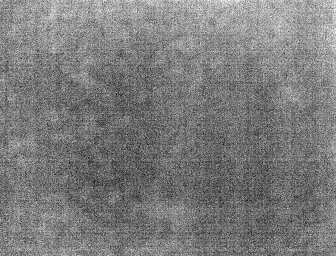
\includegraphics[width=\textwidth]{../figs/data/sea.png}
        \subcaption{Sea}
        \label{fig:sea}
    \end{subfigure}
    \hfill
    \begin{subfigure}[b]{0.49\textwidth}
        \centering
        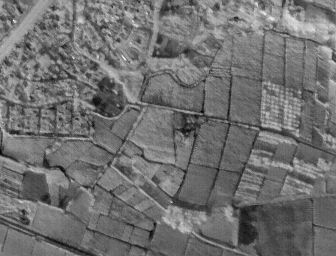
\includegraphics[width=\textwidth]{../figs/data/land.png}
        \subcaption{Land}
        \label{fig:land}
    \end{subfigure}
    \caption{A thermal image of pure sea \vs an image of land for reference.}
    \label{fig:sea_image}
\end{figure}

For both those reasons, it was decided to design a classifier for filtering out all sea images from the data.
As explained and visualized, sea images are made mostly out of a DC component and measurement noise.
This means that the gradients of two images of sea, even at different temperatures, should have a very similar high-frequency spectral content.
Analysing the gradients of sea and land images confirms this hypothesis, as can be seen in figure \ref{fig:grad_img_comp}.
\begin{figure}[H]
    \begin{subfigure}[b]{0.32\textwidth}
        \centering
        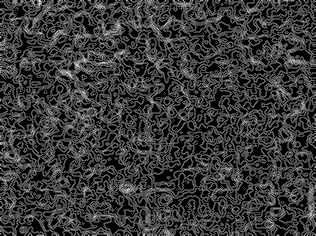
\includegraphics[width=\textwidth]{../figs/data/sea_grad-ref.png}
        \subcaption{Sea Reference}
        \label{fig:sea_grad-ref}
    \end{subfigure}
    \hfill    
    \begin{subfigure}[b]{0.32\textwidth}
        \centering
        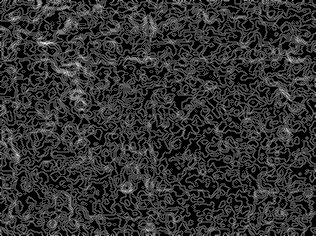
\includegraphics[width=\textwidth]{../figs/data/sea_grad.png}
        \subcaption{Sea}
        \label{fig:sea_grad}
    \end{subfigure}
    \hfill
    \begin{subfigure}[b]{0.32\textwidth}
        \centering
        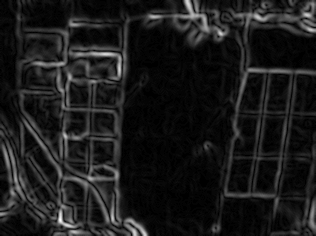
\includegraphics[width=\textwidth]{../figs/data/land_grad.png}
        \subcaption{Land}
        \label{fig:land_grad}
    \end{subfigure}
    \caption{The gradient maps of land and sea images. An additional gradient map of a sea image is provided for reference.}
    \label{fig:grad_img_comp}
\end{figure}
This finding encouraged us to base our classifier upon the gradients of the images.
A more thorough quantitative analysis of the gradients revealed a significant difference between the norm of the gradients of sea and ground images.
This difference is also demonstrated in figure \ref{fig:gradients_norm} where the norms of randomely selected sea and land images are compared
\begin{figure}[H]
    \centering
    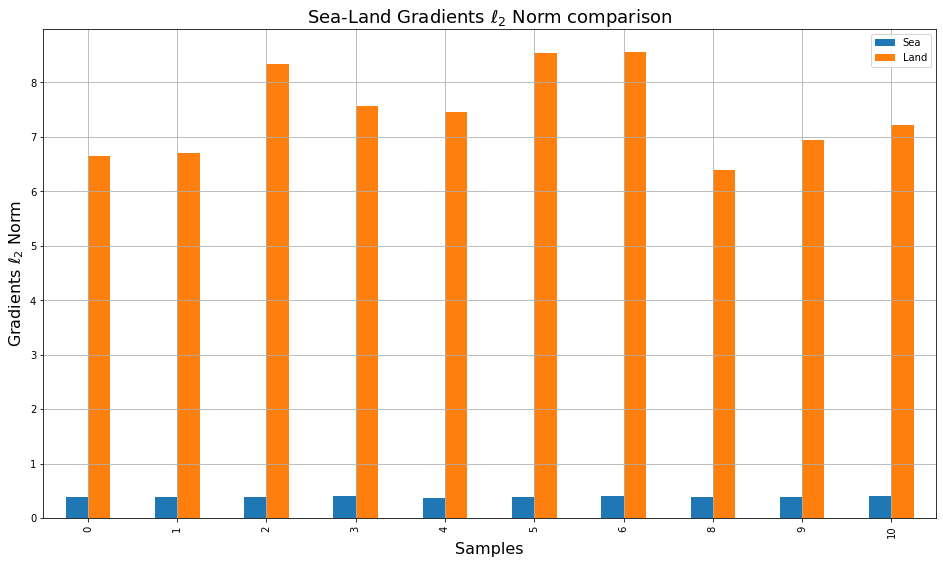
\includegraphics[width=\linewidth]{../figs/data/grad_norm_comp.png}
    \caption{A $\ell_2$ norm histogram of the gradients of random sea and images taken from the dataset.}
    \label{fig:gradients_norm}
\end{figure}

Following the findings, the following classifier was designed:
\begin{enumerate}
    \item Pre-filter the image $I$ with a gaussian low-pass filter to attenuate the noise and very high frequencies, which aren't a typical spectral content of a natural image. 
    We denote our filtered image by $\tilde{I}$.
    \item Calculate $||\nabla \tilde{I}||_2$ (the $\ell_2$ norm of the gradient of $\tilde{I}$).
    \item Compare the calculated norm to a threshold $\tau$, which dictates the eventual class prediction of the $I$.
\end{enumerate}
Where $\tau$'s value was set to the average between the minimum gradient's $\ell_2$ norm over a random set of 1000 land images and the maximum gradient's $\ell_2$ norm over a random set of 1000 sea images.
In math:
\begin{equation}
    \tau = \frac{1}{2} \left( \underset{I_\mathit{land} \in D_\mathit{land}}{min} \{||\nabla I_\mathit{land}||_2\} 
    + \underset{I_\mathit{sea} \in D_\mathit{sea}}{max} \{||\nabla I_\mathit{sea}||_2\} \right)
\end{equation}
The entire pipeline, as well as the calibrated threshold, were designed and applied to both monochromatic and panchromatic images independently.

\subsection{Image processing}
Our proposed method is based on a deep ANN architecture that can only accept quadratic images whose dimensions need to be powers of 2.
Therefore, and since the original dimensions of images taken with our camera are $256 \times 336$ pixels, a $256 \times 256$ central cropping was applied to all captured images prior to training/testing and physical model calibration.
While a common practice, random cropping couldn't be done here, since the spatial abberations incurred by the bandpass filter of the monochromatic images are significantly dependent on the relative position in the image. 
Therefore, random cropping would compromise the generator's ability to accurately predict the required abberation pattern.
This consideration was also taken into account when we considered applying additional image augmentations, which led us to categorically avoid performing any kind of spatial transformation.

As per normalization, the standard scaler approach was taken, \ie, the mean and standard deviation of each data domain (panchromatic, monochromatic) were calculated based solely on the training set, and then used to normalize the loaded images from all sets (training, validation and test).
